\documentclass[12pt,a4paper]{article}
\usepackage[top=2.5cm,bottom=2.5cm,left=2.5cm,right=2.5cm,headheight=15pt]{geometry}
\usepackage{amsmath,amssymb}
\usepackage{tikz}
\usetikzlibrary{shapes,arrows,arrows.meta,positioning,calc}
\usepackage{booktabs,array}
\usepackage{xcolor}
\usepackage{enumitem}
\usepackage{fancyhdr}
\usepackage{titlesec}
\usepackage{mdframed}
\usepackage{tcolorbox}
\tcbuselibrary{skins,breakable}
\usepackage{hyperref}

%% ---- Colors ----
\definecolor{folblue}{RGB}{0,82,165}
\definecolor{lightblue}{RGB}{220,235,255}
\definecolor{darkorange}{RGB}{180,70,0}
\definecolor{lightorange}{RGB}{255,235,210}
\definecolor{darkgreen}{RGB}{20,110,20}
\definecolor{lightgreen}{RGB}{200,240,205}
\definecolor{darkred}{RGB}{150,20,20}
\definecolor{lightred}{RGB}{255,210,210}
\definecolor{lightgray}{RGB}{242,242,242}

%% ---- tcolorbox styles ----
\newtcolorbox{qbox}[2][]{enhanced,breakable,
  colback=lightorange,colframe=darkorange,arc=4pt,
  title={\textbf{#2}},fonttitle=\bfseries\color{white},
  attach boxed title to top left={yshift=-2mm,xshift=4mm},
  boxed title style={colback=darkorange,arc=3pt},#1}

\newtcolorbox{solbox}[2][]{enhanced,breakable,
  colback=lightblue,colframe=folblue,arc=4pt,
  title={\textbf{#2}},fonttitle=\bfseries\color{white},
  attach boxed title to top left={yshift=-2mm,xshift=4mm},
  boxed title style={colback=folblue,arc=3pt},#1}

\newtcolorbox{keybox}[2][]{enhanced,breakable,
  colback=lightgreen,colframe=darkgreen,arc=4pt,
  title={\textbf{#2}},fonttitle=\bfseries\color{white},
  attach boxed title to top left={yshift=-2mm,xshift=4mm},
  boxed title style={colback=darkgreen,arc=3pt},#1}

\newtcolorbox{algobox}[2][]{enhanced,breakable,
  colback=lightgray,colframe=gray!60,arc=4pt,
  title={\textbf{#2}},fonttitle=\bfseries,
  attach boxed title to top left={yshift=-2mm,xshift=4mm},
  boxed title style={colback=gray!60,arc=3pt},#1}

\newtcolorbox{warnbox}[2][]{enhanced,breakable,
  colback=lightred,colframe=darkred,arc=4pt,
  title={\textbf{#2}},fonttitle=\bfseries\color{white},
  attach boxed title to top left={yshift=-2mm,xshift=4mm},
  boxed title style={colback=darkred,arc=3pt},#1}

%% ---- Page style ----
\pagestyle{fancy}\fancyhf{}
\lhead{\color{folblue}\textbf{IPsec --- CSE 717 InfoSec}}
\rhead{\color{folblue}Exam: 17 Jun 2026}
\cfoot{--- \thepage\ ---}
\renewcommand{\headrulewidth}{0.4pt}

%% ---- Section style ----
\titleformat{\section}{\large\bfseries\color{folblue}}{}{0em}{}[\titlerule]
\titleformat{\subsection}{\normalsize\bfseries\color{darkorange}}{}{0em}{}

\begin{document}

\begin{center}
  {\LARGE\bfseries\color{folblue} IPsec (IP Security)}\\[4pt]
  {\large CSE 717 Information Security --- Past-Paper Solutions (2020, 2021, 2024)}\\[2pt]
  {\small Source: Lc\#7 pp.\,14--21 \quad Yield: 3/5 years (2020, 2021, 2024), 2.25--9 marks}
\end{center}
\vspace{0.5em}

%% ================================================================
\section{Cheat Sheet}
%% ================================================================

\begin{keybox}{IPsec Architecture --- 7 Components}
\begin{enumerate}[nosep,leftmargin=1.5em]
  \item \textbf{Architecture} --- general concepts, definitions, protocols, algorithms, security requirements
  \item \textbf{ESP Protocol} (Encapsulation Security Payload) --- provides \textbf{Confidentiality} service
  \item \textbf{Encryption Algorithm} --- documents describing algorithms used for ESP
  \item \textbf{AH Protocol} (Authentication Header) --- provides \textbf{Authentication + Integrity} services
  \item \textbf{Authentication Algorithm} --- documents for auth algorithm used by AH and auth option of ESP
  \item \textbf{DOI} (Domain of Interpretation) --- identifier supporting both AH and ESP; contains values needed for documentation
  \item \textbf{Key Management} --- describes how keys are exchanged between sender and receiver
\end{enumerate}

\medskip
\textbf{Three services provided:} Confidentiality \quad Authentication \quad Integrity
\end{keybox}

\vspace{0.5em}

\begin{algobox}{IPsec Architecture Diagram (Lc\#7 Slide 16)}
\begin{center}
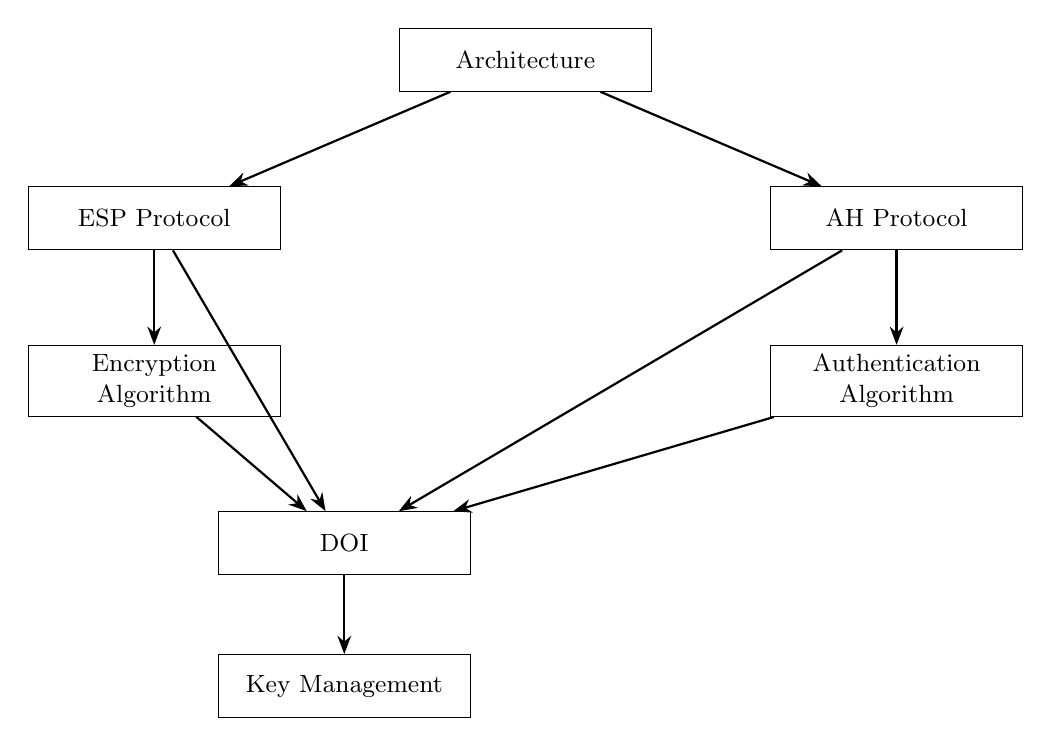
\begin{tikzpicture}[
  box/.style={rectangle, draw, minimum width=3.2cm, minimum height=0.8cm, align=center, font=\small},
  arr/.style={->,>=Stealth,thick}
]
\node[box] (arch) {Architecture};
\node[box, below left=1.2cm and 1.5cm of arch]  (esp) {ESP Protocol};
\node[box, below right=1.2cm and 1.5cm of arch] (ah)  {AH Protocol};
\node[box, below=1.2cm of esp]  (enc) {Encryption\\Algorithm};
\node[box, below=1.2cm of ah]   (aut) {Authentication\\Algorithm};
\node[box, below right=1.2cm and -0.8cm of enc] (doi) {DOI};
\node[box, below=1.0cm of doi]  (km)  {Key Management};

\draw[arr] (arch) -- (esp);
\draw[arr] (arch) -- (ah);
\draw[arr] (esp)  -- (enc);
\draw[arr] (ah)   -- (aut);
\draw[arr] (esp)  -- (doi);
\draw[arr] (enc)  -- (doi);
\draw[arr] (ah)   -- (doi);
\draw[arr] (aut)  -- (doi);
\draw[arr] (doi)  -- (km);
\end{tikzpicture}
\end{center}
\end{algobox}

\vspace{0.5em}

\begin{algobox}{Security Associations (SA)}
A \textbf{Security Association (SA)} is a one-way logical connection between communicating endpoints that provides security services for traffic carried on it.

\medskip
\textbf{An SA is uniquely identified by three parameters:}
\begin{enumerate}[nosep]
  \item \textbf{SPI} (Security Parameters Index) --- a 32-bit identifier in the AH/ESP header
  \item \textbf{Destination IP Address} --- unicast address of the receiving endpoint
  \item \textbf{Security Protocol Identifier} --- AH or ESP
\end{enumerate}

\medskip
\textbf{One-way nature:} Each SA is unidirectional. For bidirectional secure communication between two hosts, \textbf{two SAs} are required (one in each direction).

\medskip
\textbf{SA contains:} sequence number counter, anti-replay window, AH/ESP algorithm + keys, IPsec protocol mode (transport/tunnel), SA lifetime.
\end{algobox}

\vspace{0.5em}

\begin{algobox}{Transport Mode vs Tunnel Mode}
\begin{tabular}{@{}p{3.5cm}p{5.5cm}p{5cm}@{}}
\toprule
 & \textbf{Transport Mode} & \textbf{Tunnel Mode} \\
\midrule
\textbf{What it protects} & IP payload only & Entire original IP packet \\
\textbf{IP header} & Original header unchanged & New outer IP header added \\
\textbf{Use case} & End-to-end between two hosts & Gateway-to-gateway (VPN) \\
\textbf{Overhead} & Lower & Higher (extra IP header) \\
\bottomrule
\end{tabular}
\end{algobox}

\vspace{0.5em}

\begin{algobox}{RFC 4301 Services (6 Security Services)}
\begin{enumerate}[nosep]
  \item \textbf{Access control} --- controls which packets are allowed through
  \item \textbf{Connectionless integrity} --- detects modification of individual IP datagrams
  \item \textbf{Data origin authentication} --- verifies identity of the sender
  \item \textbf{Rejection of replayed packets (anti-replay)} --- detects and rejects replayed datagrams via sequence number
  \item \textbf{Confidentiality (encryption)} --- encrypts IP payload
  \item \textbf{Limited traffic flow confidentiality} --- limits exposure of traffic patterns (in tunnel mode)
\end{enumerate}
\end{algobox}

\vspace{0.5em}

\begin{algobox}{Application Areas of IPsec}
\begin{enumerate}[nosep]
  \item \textbf{Secure branch-office connectivity} (site-to-site VPN) --- securely connects remote offices over the Internet
  \item \textbf{Secure remote access} (remote-access VPN) --- employees access corporate network from home/travel
  \item \textbf{Extranet / partner connectivity} --- secure B2B communication with trading partners
  \item \textbf{Enhanced e-commerce security} --- protects transactions between customers and servers
\end{enumerate}
\end{algobox}

\vspace{1em}

%% ================================================================
\section{2024 Exam (Q5(c) --- 3 marks)}
%% ================================================================

\subsection{Section B Q5(c) --- 3 marks: Architecture + Security Associations}

\begin{qbox}{2024 Section B Q5(c) [3 marks]}
  Explain the IPsec architecture and the role of security associations.
\end{qbox}

\begin{solbox}{Solution}
\textbf{IPsec Architecture:}

IPsec (IP Security) architecture uses two protocols to secure data flow:
\begin{itemize}[nosep]
  \item \textbf{ESP} (Encapsulation Security Payload) --- provides \textbf{confidentiality}
  \item \textbf{AH} (Authentication Header) --- provides \textbf{authentication and integrity}
\end{itemize}

The architecture includes four supporting documents:
\begin{itemize}[nosep]
  \item \textbf{Encryption Algorithm} --- describes encryption for ESP
  \item \textbf{Authentication Algorithm} --- describes auth algorithm for AH and ESP
  \item \textbf{DOI} (Domain of Interpretation) --- identifier supporting both AH and ESP
  \item \textbf{Key Management} --- describes key exchange between sender and receiver
\end{itemize}

\bigskip
\textbf{Role of Security Associations (SA):}

A \textbf{Security Association} is a one-way logical connection that defines the security parameters for traffic between two endpoints. It is uniquely identified by:
\begin{enumerate}[nosep]
  \item SPI (Security Parameters Index)
  \item Destination IP address
  \item Security protocol (AH or ESP)
\end{enumerate}

An SA is \textbf{unidirectional} --- two SAs are needed for bidirectional communication. Each SA specifies the cryptographic algorithm, keys, and mode (transport or tunnel) to be used.
\end{solbox}

\vspace{1em}

%% ================================================================
\section{2021 Exam (Q4(b,c) --- 5 marks total)}
%% ================================================================

\subsection{Section B Q4(b) --- 2.5 marks: Application Areas + Session vs Connection State}

\begin{qbox}{2021 Section B Q4(b) [2.5 marks]}
  Describe the application areas of IPsec and explain the distinction between session state and connection state in IPsec.
\end{qbox}

\begin{solbox}{Solution}
\textbf{Application Areas of IPsec:}
\begin{enumerate}[nosep]
  \item \textbf{Secure branch-office connectivity} --- IPsec tunnel mode connects remote offices to HQ over the Internet, creating a site-to-site VPN.
  \item \textbf{Secure remote access} --- remote employees use IPsec to access internal corporate resources securely from home or while traveling.
  \item \textbf{Extranet/partner connectivity} --- businesses use IPsec to securely communicate with trading partners.
  \item \textbf{Enhanced e-commerce} --- protects financial transactions and customer data.
\end{enumerate}

\bigskip
\textbf{Session State vs Connection State:}
\begin{itemize}[nosep]
  \item A \textbf{connection} refers to the state maintained for a single one-way IP flow protected by a specific Security Association (SA). Each SA has its own sequence numbers, keys, and lifetime.
  \item A \textbf{session} is a higher-level concept representing bidirectional communication between two parties. Since each SA is one-way, a session requires \textbf{two connections (two SAs)}.
  \item IPsec operates at the IP (network) layer and is \textbf{connectionless} at the packet level --- each packet is individually secured based on the SA, without requiring a persistent TCP-style connection.
\end{itemize}
\end{solbox}

\vspace{1em}

\subsection{Section B Q4(c) --- 2.5 marks: Architecture}

\begin{qbox}{2021 Section B Q4(c) [2.5 marks]}
  Describe the IPsec architecture.
\end{qbox}

\begin{solbox}{Solution}
\textbf{IPsec Architecture} provides security services at the IP layer using two protocols and four supporting documents:

\medskip
\textbf{Protocols:}
\begin{itemize}[nosep]
  \item \textbf{ESP (Encapsulation Security Payload)} --- encrypts the IP payload to provide confidentiality.
  \item \textbf{AH (Authentication Header)} --- provides authentication and integrity without encryption.
\end{itemize}

\medskip
\textbf{Supporting Documents:}
\begin{itemize}[nosep]
  \item \textbf{Encryption Algorithm} --- specifies encryption algorithms used with ESP.
  \item \textbf{Authentication Algorithm} --- specifies auth algorithms for AH and the auth option of ESP.
  \item \textbf{DOI (Domain of Interpretation)} --- identifier that supports both AH and ESP; contains values for cross-referencing security parameters.
  \item \textbf{Key Management} --- documents how session keys are securely exchanged between communicating parties.
\end{itemize}

\medskip
Together these components provide three core services: \textbf{confidentiality}, \textbf{authentication}, and \textbf{integrity}.
\end{solbox}

\vspace{1em}

%% ================================================================
\section{2020 Exam (Q8 --- 8.75 marks total)}
%% ================================================================

\subsection{Q8(a) --- 2.25 marks: Benefits + Transport vs Tunnel Mode}

\begin{qbox}{2020 Q8(a) [2.25 marks]}
  What are the benefits of IPsec? Explain transport mode and tunnel mode.
\end{qbox}

\begin{solbox}{Solution}
\textbf{Benefits of IPsec:}
\begin{itemize}[nosep]
  \item \textbf{Confidentiality} --- encrypts data so eavesdroppers cannot read it (via ESP).
  \item \textbf{Authentication} --- verifies the sender's identity (via AH or ESP auth option).
  \item \textbf{Integrity} --- ensures data is not tampered with in transit.
  \item \textbf{Anti-replay protection} --- prevents replay attacks via sequence numbers.
  \item \textbf{Access control} --- filters which traffic is permitted through the gateway.
\end{itemize}

\bigskip
\textbf{Transport Mode:}
\begin{itemize}[nosep]
  \item Protects only the \textbf{IP payload} (not the original IP header).
  \item The original IP header is left unchanged and transmitted as-is.
  \item Used for \textbf{end-to-end} communication between two hosts.
  \item Lower overhead.
\end{itemize}

\textbf{Tunnel Mode:}
\begin{itemize}[nosep]
  \item Encapsulates the \textbf{entire original IP packet} (header + payload) inside a new IP packet.
  \item A new outer IP header is added, hiding the original source/destination.
  \item Used for \textbf{gateway-to-gateway} VPN (site-to-site tunnels).
  \item Higher overhead but provides full original packet protection.
\end{itemize}
\end{solbox}

\vspace{1em}

\subsection{Q8(b) --- 2.25 marks: RFC 4301 Services}

\begin{qbox}{2020 Q8(b) [2.25 marks]}
  List and explain the security services defined by RFC 4301 for IPsec.
\end{qbox}

\begin{solbox}{Solution}
RFC 4301 defines \textbf{six security services} for IPsec:
\begin{enumerate}[nosep]
  \item \textbf{Access control} --- enforces policy on which IP traffic is allowed (discard, bypass, or protect).
  \item \textbf{Connectionless integrity} --- detects modification of individual IP datagrams without requiring a persistent connection.
  \item \textbf{Data origin authentication} --- verifies that the packet came from the claimed source.
  \item \textbf{Rejection of replayed packets (anti-replay)} --- uses a sliding window and sequence numbers to detect and drop replayed datagrams.
  \item \textbf{Confidentiality (encryption)} --- encrypts the contents of IP packets so only authorized parties can read them (provided by ESP).
  \item \textbf{Limited traffic flow confidentiality} --- conceals traffic patterns (e.g., source/destination) in tunnel mode.
\end{enumerate}
\end{solbox}

\vspace{1em}

\subsection{Q8(c) --- 2.25 marks: Application Areas + Session/Connection State}

\begin{qbox}{2020 Q8(c) [2.25 marks]}
  What are the application areas of IPsec? Explain session state and connection state.
\end{qbox}

\begin{solbox}{Solution}
\textbf{Application Areas:}
\begin{enumerate}[nosep]
  \item Secure branch-office connectivity (site-to-site VPN)
  \item Secure remote access VPN for employees
  \item Secure B2B extranet connections with trading partners
  \item Enhanced e-commerce security for customer transactions
\end{enumerate}

\bigskip
\textbf{Session State vs Connection State:}
\begin{itemize}[nosep]
  \item \textbf{Connection state:} maintained per Security Association (SA). Each SA stores: SPI, sequence number counter, anti-replay window, cryptographic keys, SA lifetime, and mode (transport/tunnel). One SA = one unidirectional connection.
  \item \textbf{Session state:} a logical grouping of two SAs (one in each direction) forming a bidirectional secure session between two entities.
  \item IPsec itself is \textbf{stateless at the packet level} (each datagram processed independently based on the SA), but the SA database (SAD) holds connection state that persists for the SA's lifetime.
\end{itemize}
\end{solbox}

\vspace{1em}

\subsection{Q8(d) --- 2 marks: Architecture}

\begin{qbox}{2020 Q8(d) [2 marks]}
  Draw and explain the IPsec architecture.
\end{qbox}

\begin{solbox}{Solution}
\textbf{IPsec Architecture} (per Lc\#7 Slide 16):

\begin{center}
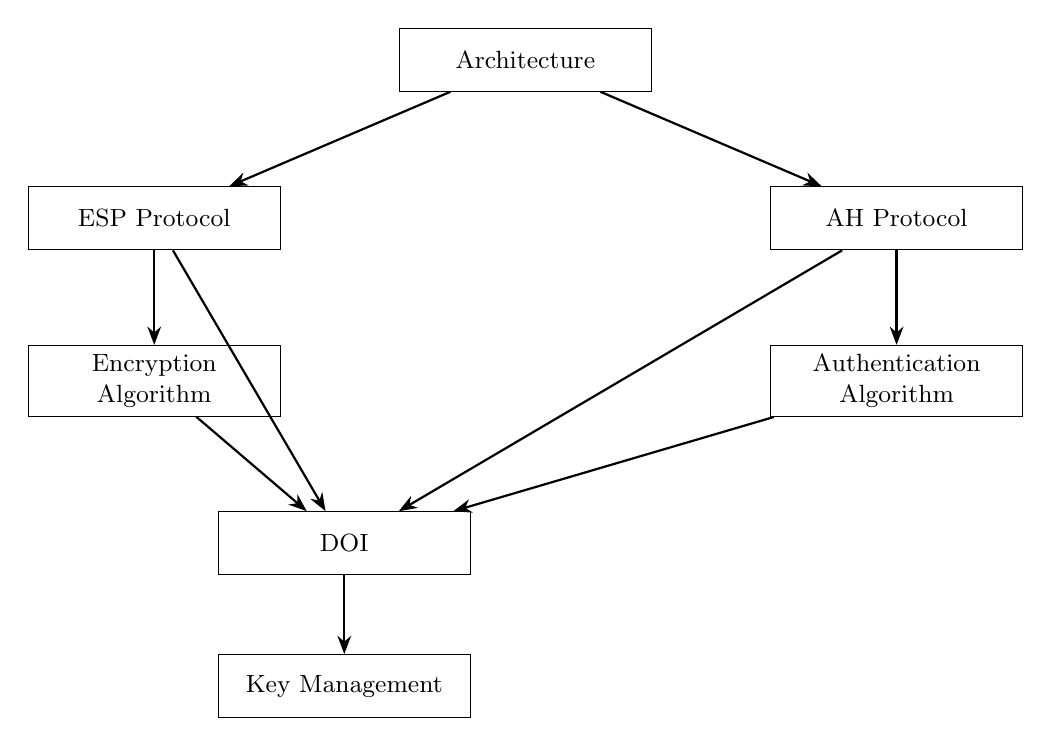
\begin{tikzpicture}[
  box/.style={rectangle, draw, minimum width=3.2cm, minimum height=0.8cm, align=center, font=\small},
  arr/.style={->,>=Stealth,thick}
]
\node[box] (arch) {Architecture};
\node[box, below left=1.2cm and 1.5cm of arch]  (esp) {ESP Protocol};
\node[box, below right=1.2cm and 1.5cm of arch] (ah)  {AH Protocol};
\node[box, below=1.2cm of esp]  (enc) {Encryption\\Algorithm};
\node[box, below=1.2cm of ah]   (aut) {Authentication\\Algorithm};
\node[box, below right=1.2cm and -0.8cm of enc] (doi) {DOI};
\node[box, below=1.0cm of doi]  (km)  {Key Management};

\draw[arr] (arch) -- (esp);
\draw[arr] (arch) -- (ah);
\draw[arr] (esp)  -- (enc);
\draw[arr] (ah)   -- (aut);
\draw[arr] (esp)  -- (doi);
\draw[arr] (enc)  -- (doi);
\draw[arr] (ah)   -- (doi);
\draw[arr] (aut)  -- (doi);
\draw[arr] (doi)  -- (km);
\end{tikzpicture}
\end{center}

\begin{itemize}[nosep]
  \item \textbf{Architecture} --- top-level document covering general concepts and security requirements
  \item \textbf{ESP Protocol} --- confidentiality; \textbf{AH Protocol} --- authentication + integrity
  \item \textbf{Encryption / Authentication Algorithm} --- document sets for the respective protocols
  \item \textbf{DOI} --- shared identifier binding AH and ESP to common parameter values
  \item \textbf{Key Management} --- IKE (Internet Key Exchange) protocol for establishing and managing SAs
\end{itemize}
\end{solbox}

\vspace{1em}

%% ================================================================
\section{Exam Strategy}
%% ================================================================

\begin{keybox}{Recurring Sub-Question Cluster (2020, 2021, 2024)}
\begin{tabular}{@{}llll@{}}
\toprule
\textbf{Sub-question} & \textbf{2020} & \textbf{2021} & \textbf{2024} \\
\midrule
Architecture (diagram + explanation) & Q8(d) 2m & Q4(c) 2.5m & Q5(c) 3m \\
Transport vs Tunnel mode & Q8(a) 2.25m & --- & --- \\
RFC 4301 services & Q8(b) 2.25m & --- & --- \\
Application areas & Q8(c) 2.25m & Q4(b) 2.5m & --- \\
Session vs connection state & Q8(c) 2.25m & Q4(b) 2.5m & --- \\
Security Associations & --- & --- & Q5(c) 3m \\
\bottomrule
\end{tabular}

\medskip
\textbf{Architecture} is the most reliable repeat (appears 2020, 2021, 2024 --- all 3 years). Draw the diagram even if not explicitly asked.

\medskip
\textbf{Mnemonics:}
\begin{itemize}[nosep]
  \item \textbf{ESP = Encrypt} (E = Encrypt); \textbf{AH = Auth + Integrity} (A = Auth)
  \item RFC 4301 services: \textbf{ACC-D-RC} --- Access control, Connectionless integrity, data origin auth, Duplicate/replay rejection, Confidentiality, traffic flow Confidentiality (limited)
\end{itemize}
\end{keybox}

\end{document}
